\chapter{Appendix}\label{appendix}

\section{N-grams WordClouds}\label{appendix:ngrams}

\begin{figure}[H]
    \centering
    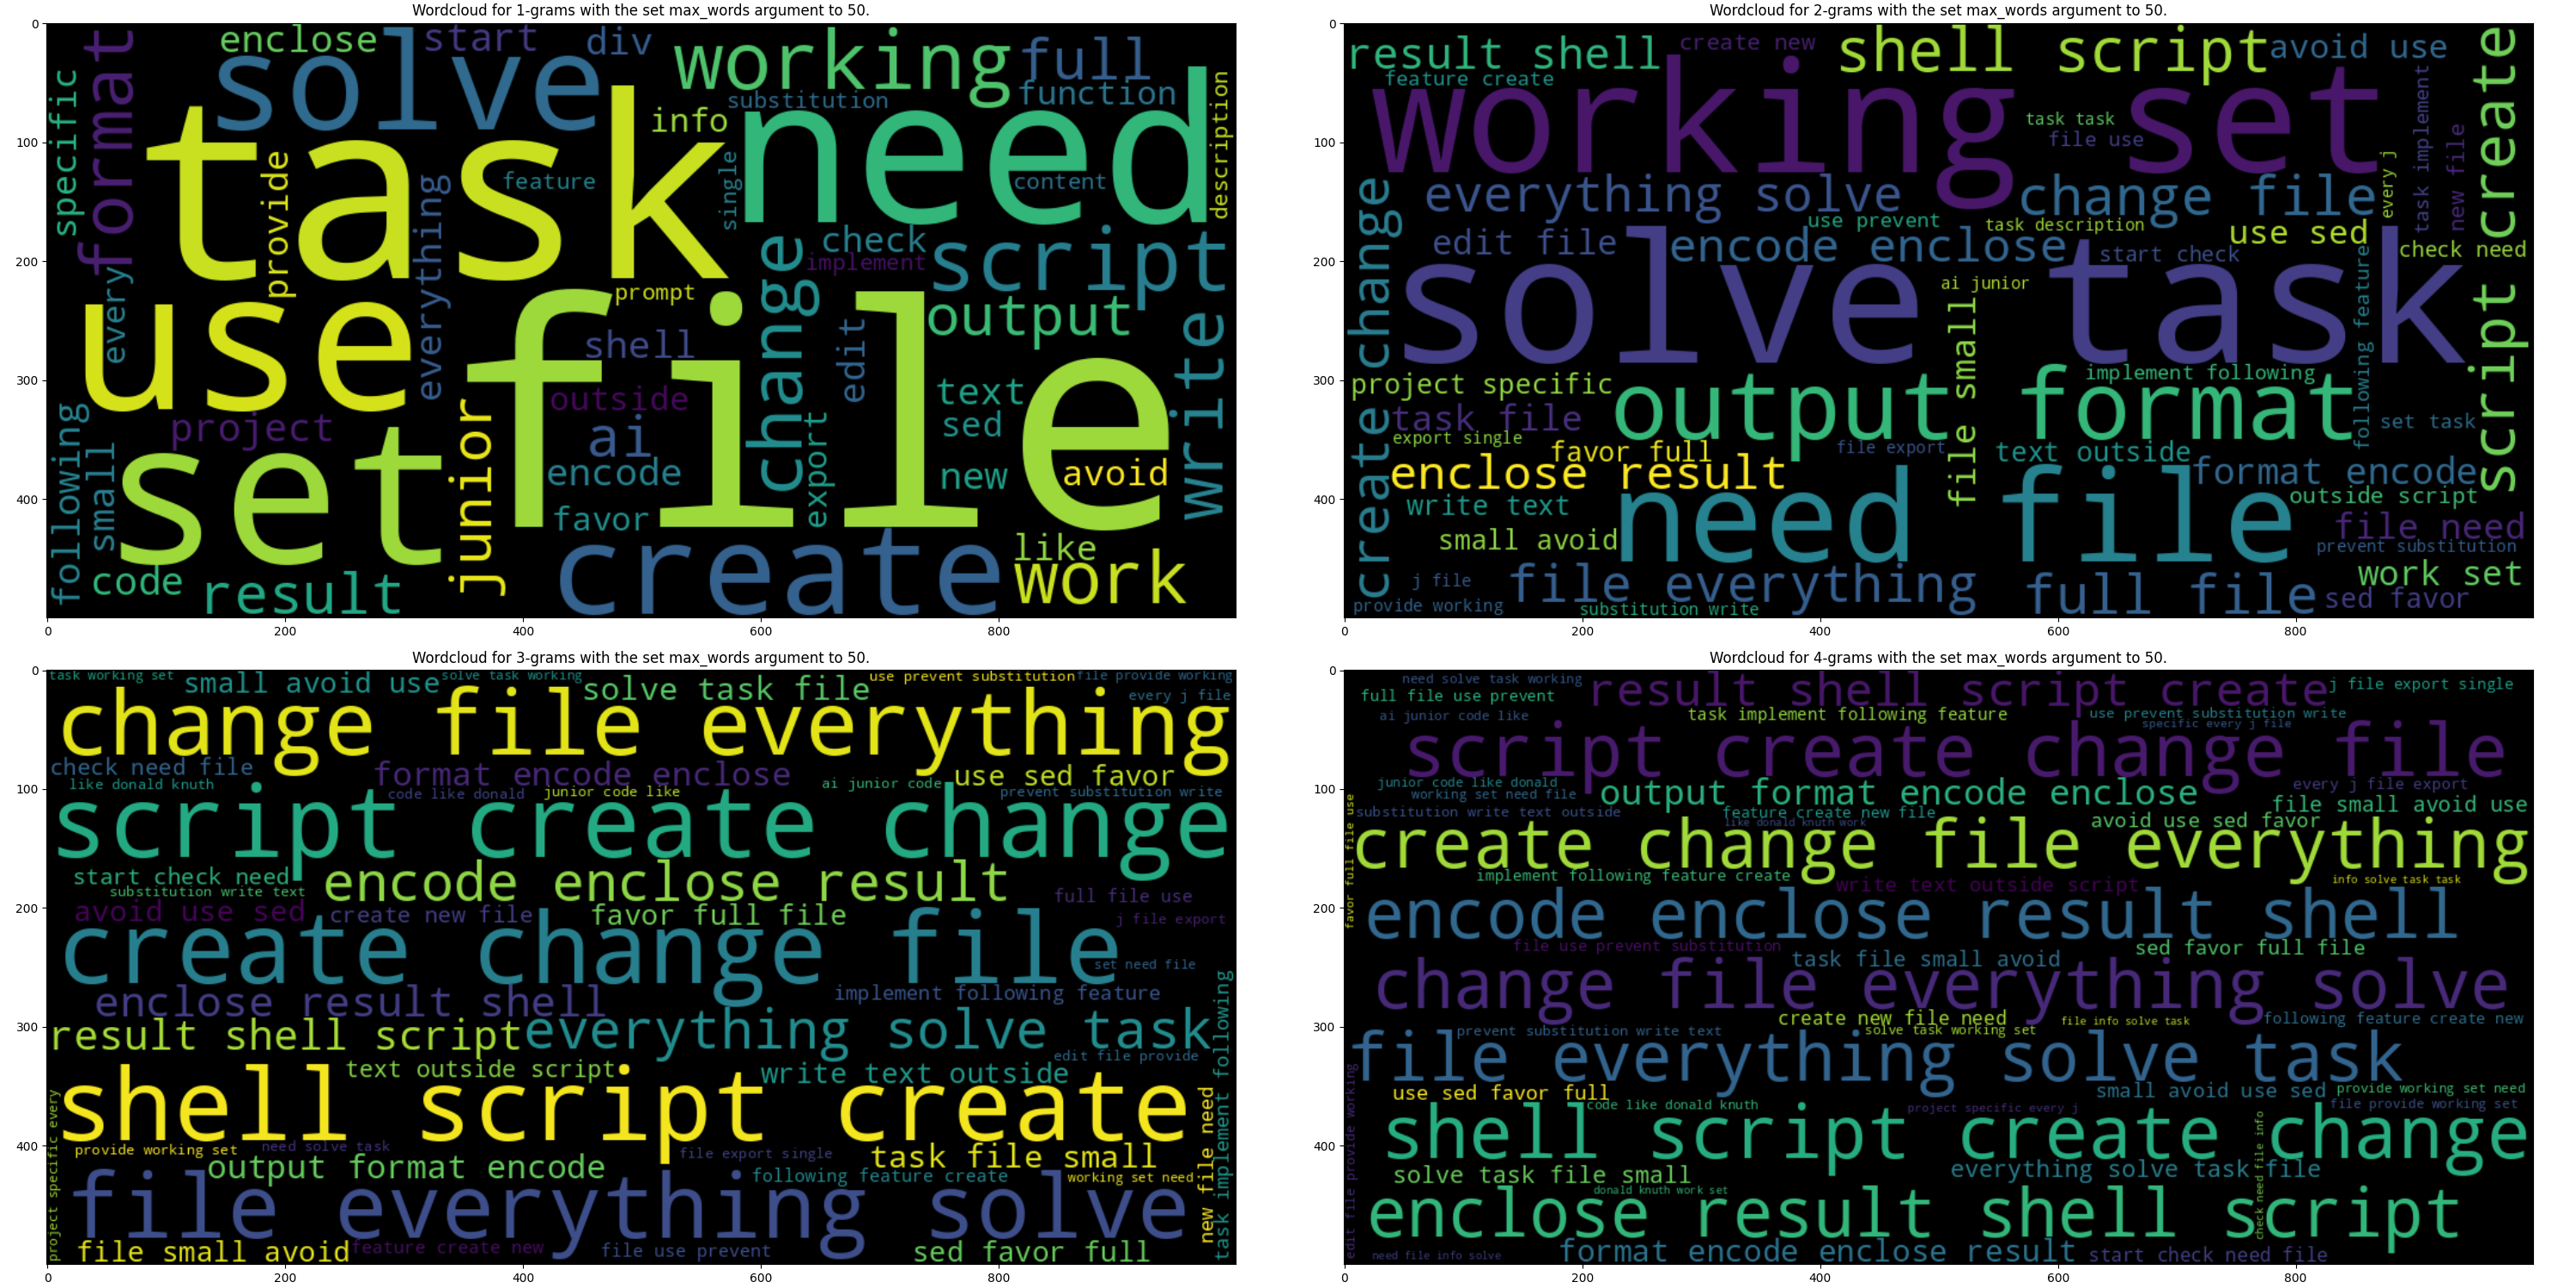
\includegraphics[width=\textwidth]{imgs/commits-ngrams.png}
    \caption{N-grams from conversations sourced from GitHub commits.}
    \label{fig:commits-ngrams}
\end{figure}

\begin{figure}[H]
    \centering
    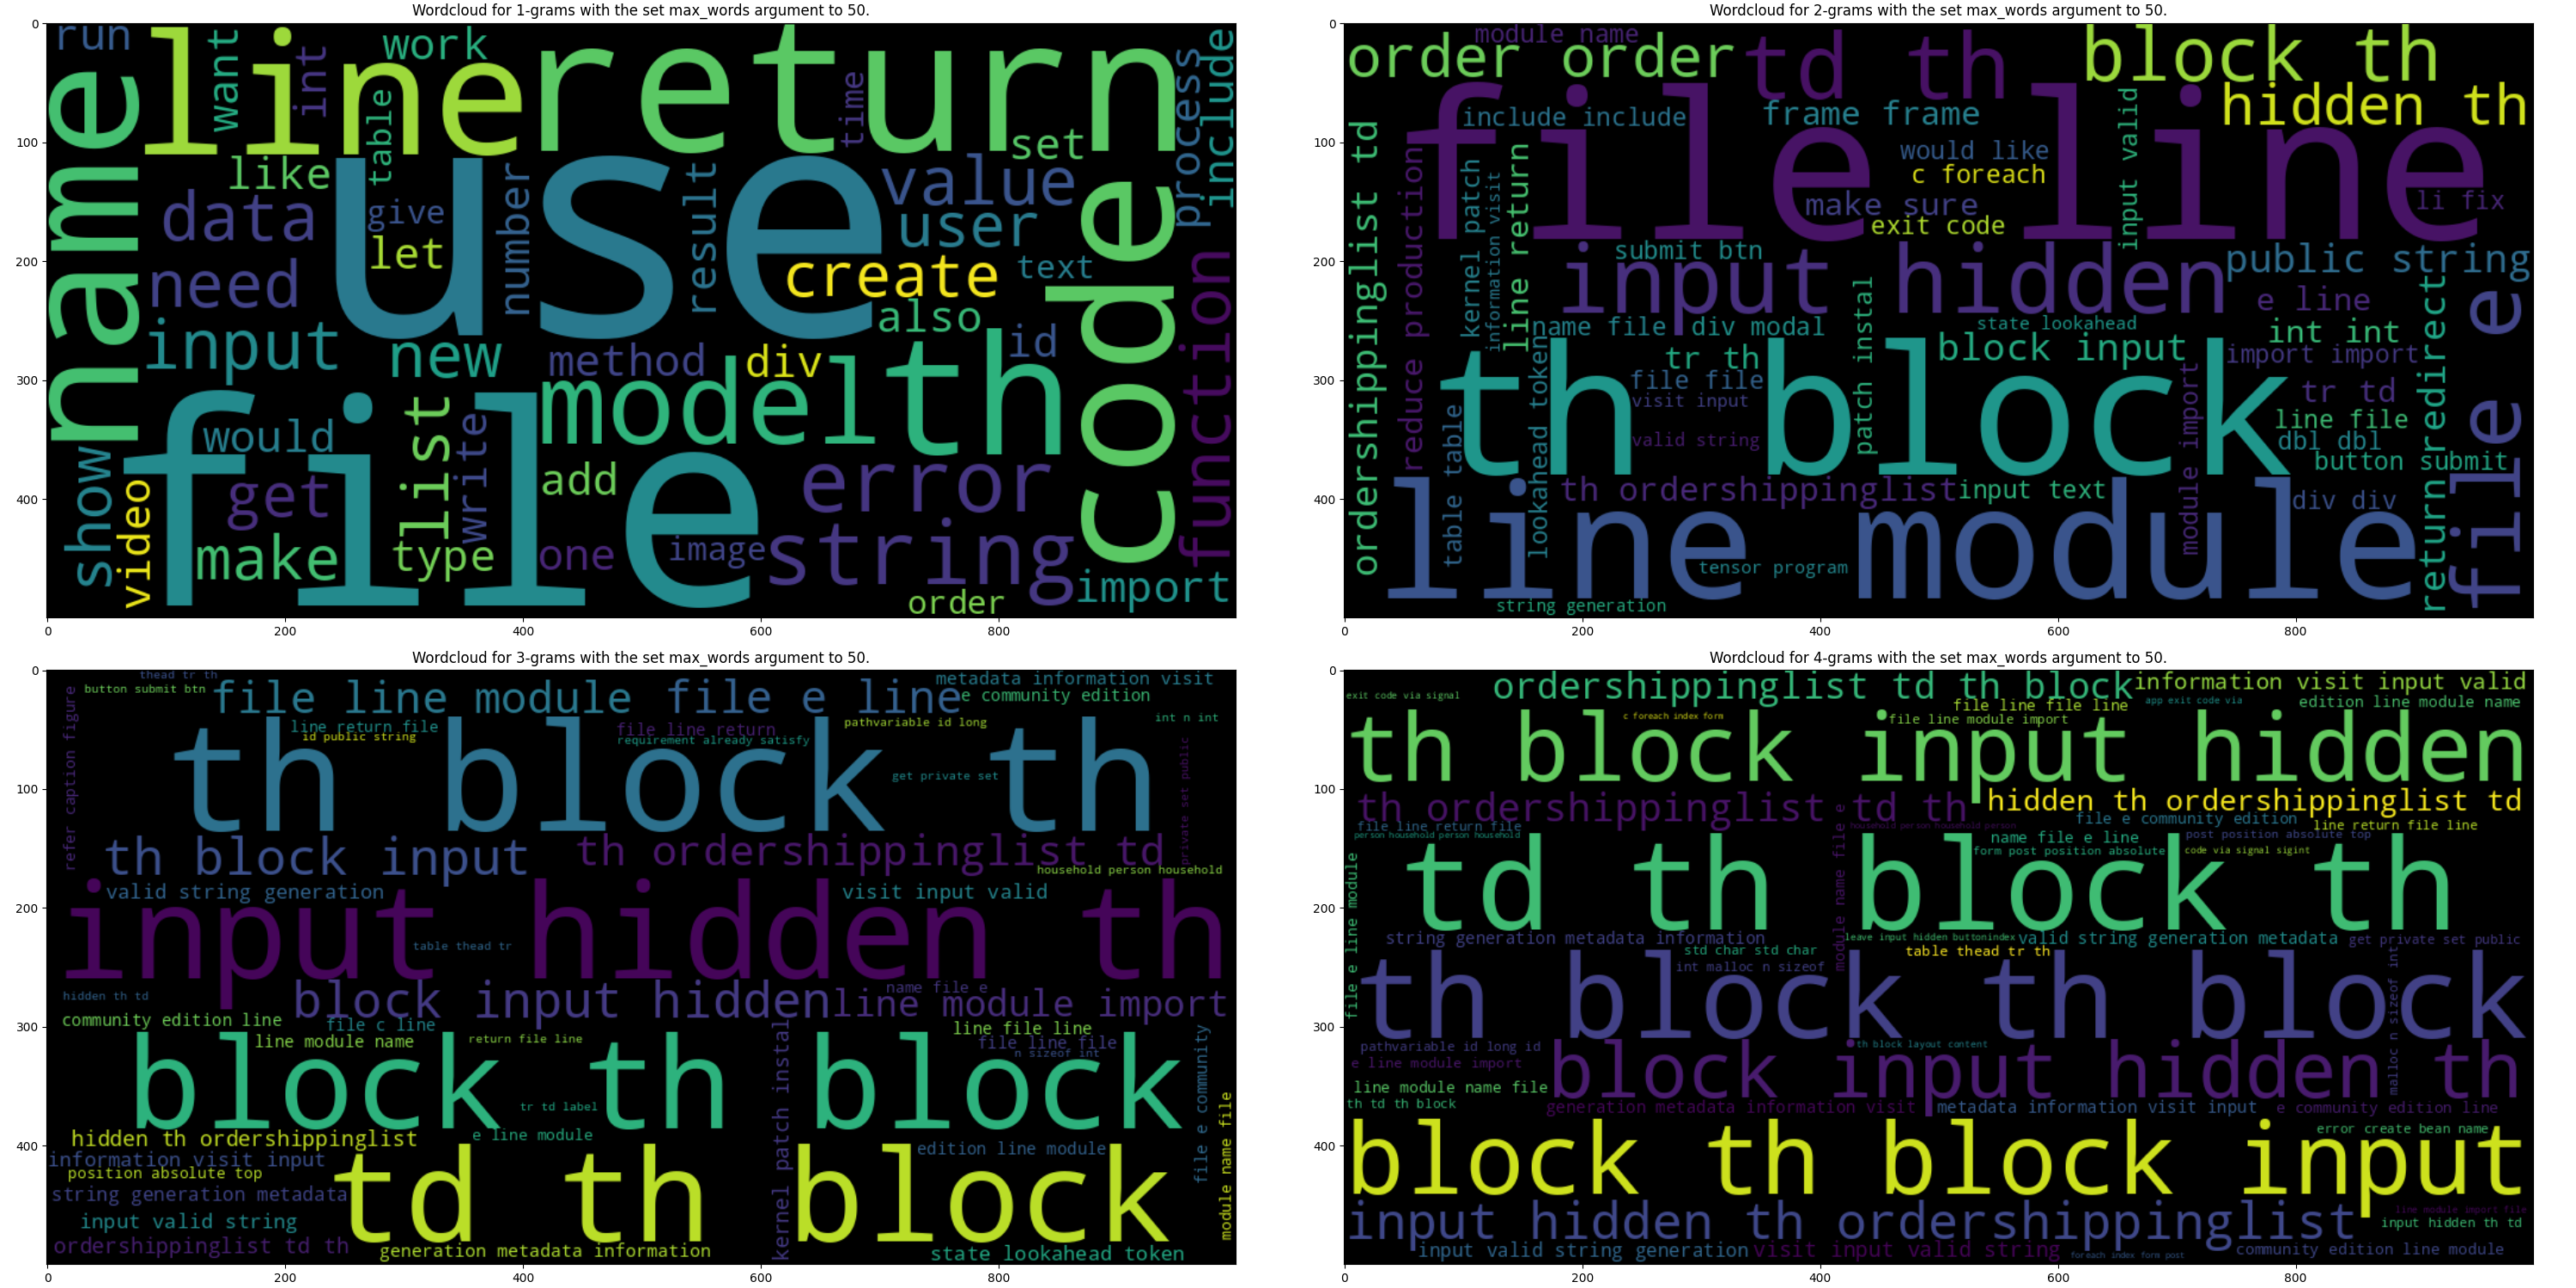
\includegraphics[width=\textwidth]{imgs/issues-ngrams.png}
    \caption{N-grams from conversations sourced from GitHub issues.}
    \label{fig:issues-ngrams}
\end{figure}

\begin{figure}[H]
    \centering
    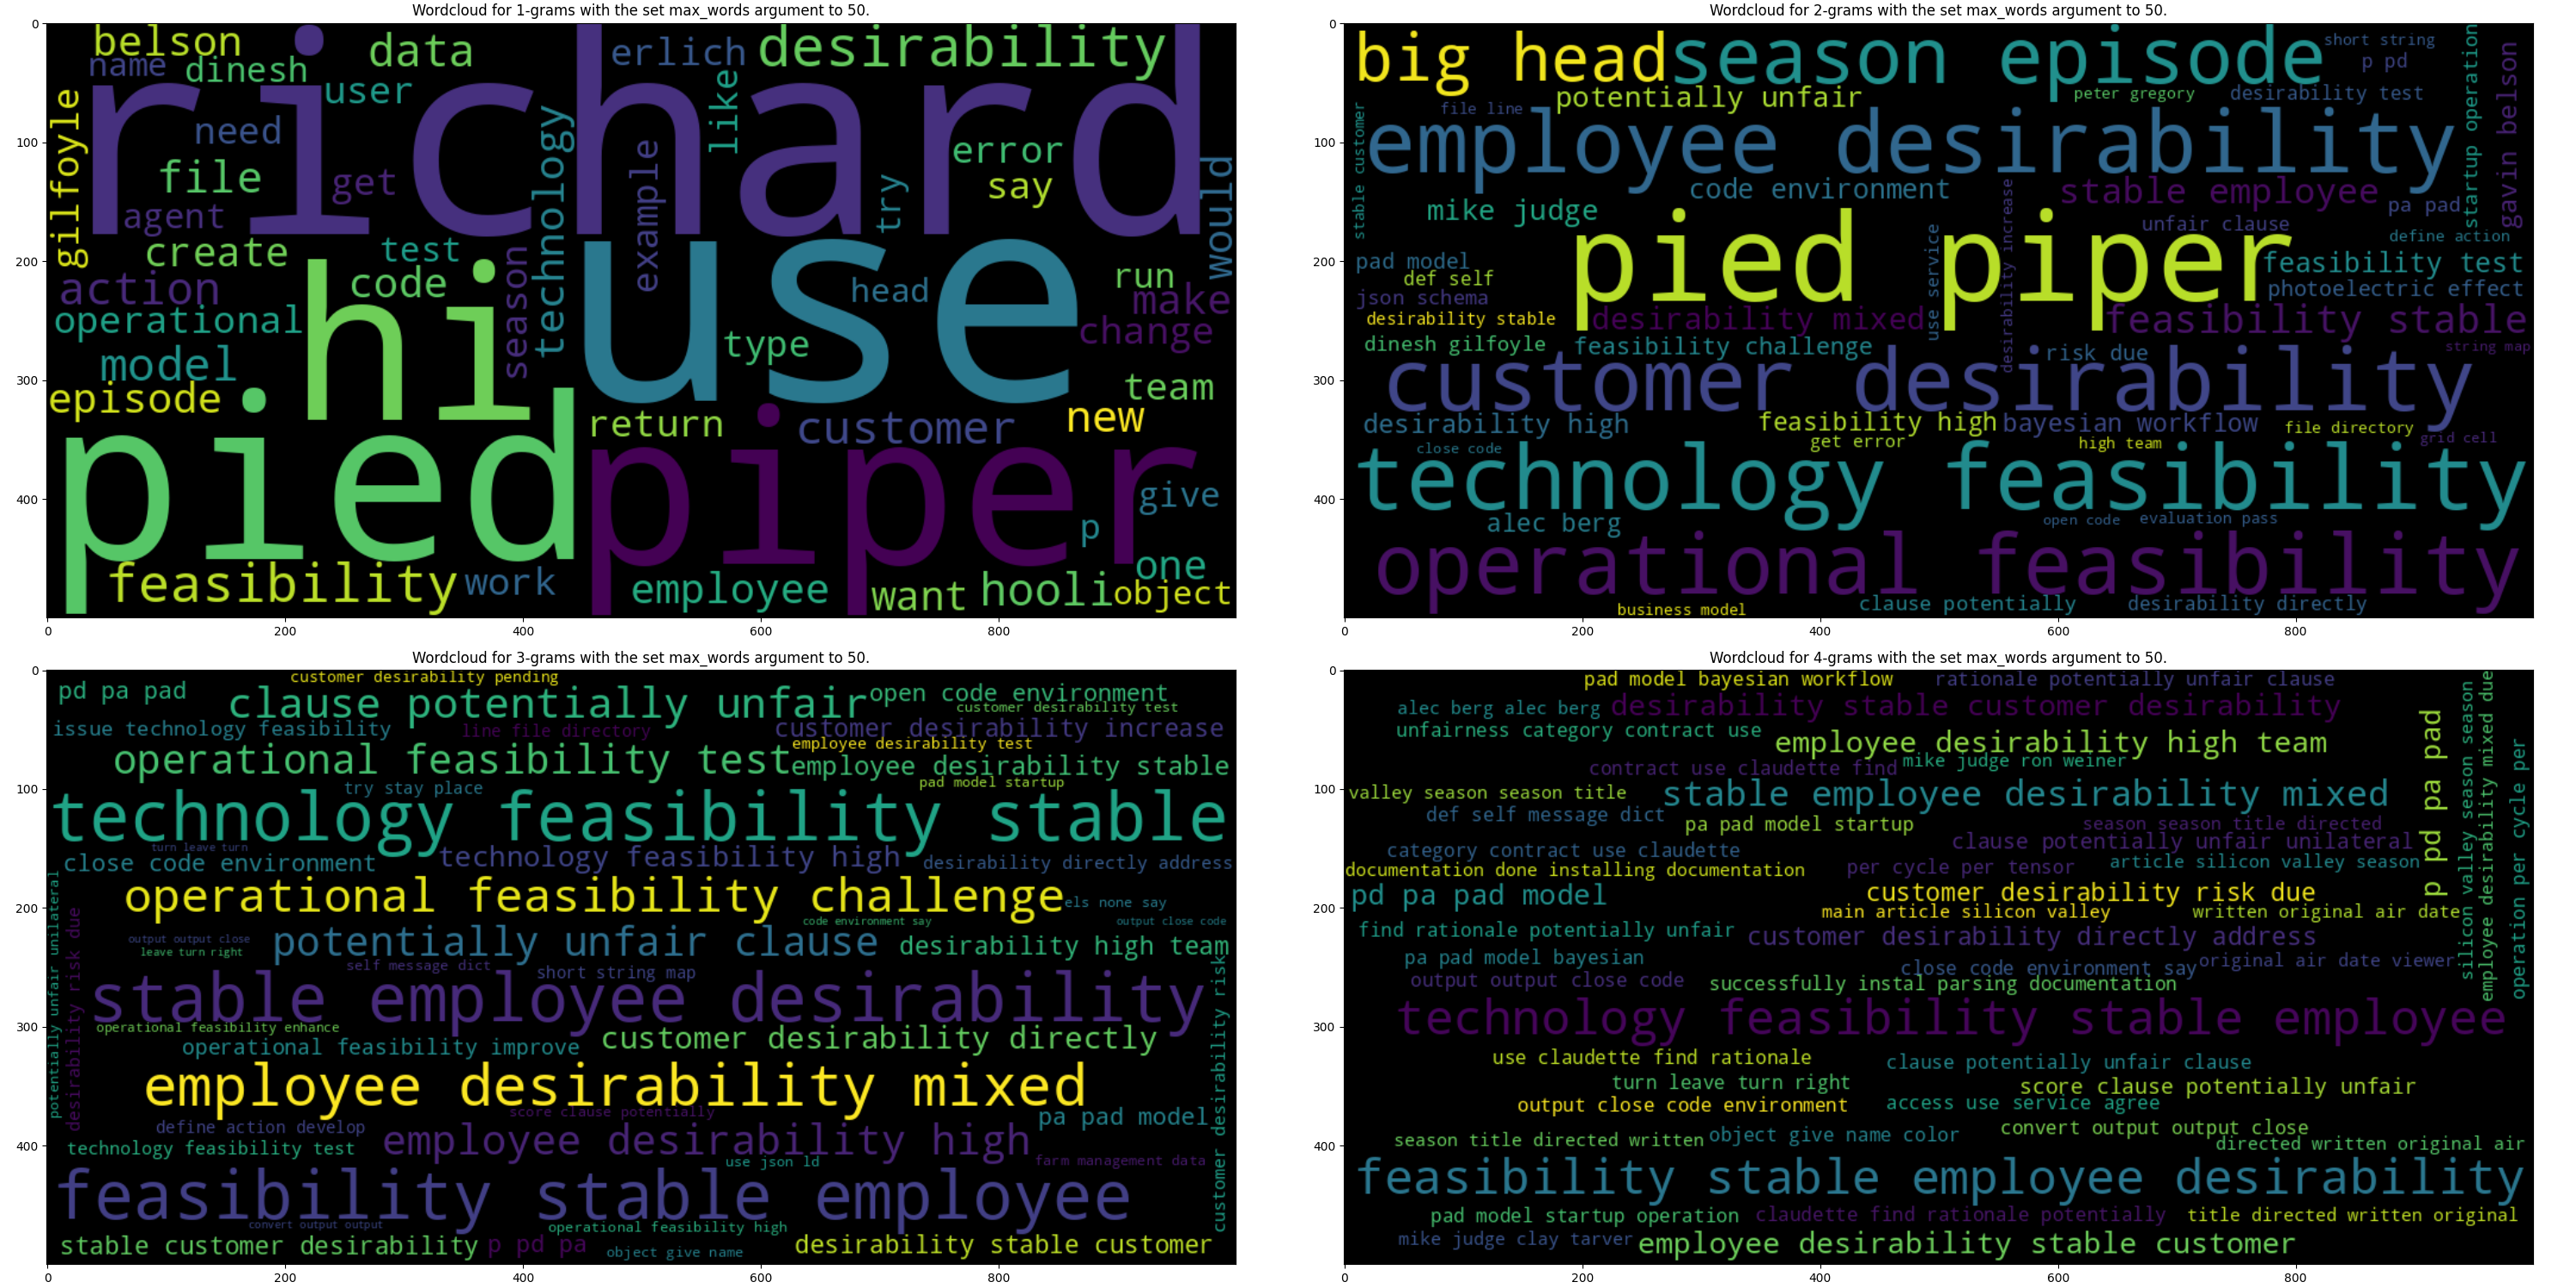
\includegraphics[width=\textwidth]{imgs/discussions-ngrams.png}
    \caption{N-grams from conversations sourced from GitHub discussions.}
    \label{fig:discussions-ngrams}
\end{figure}

\begin{figure}[H]
    \centering
    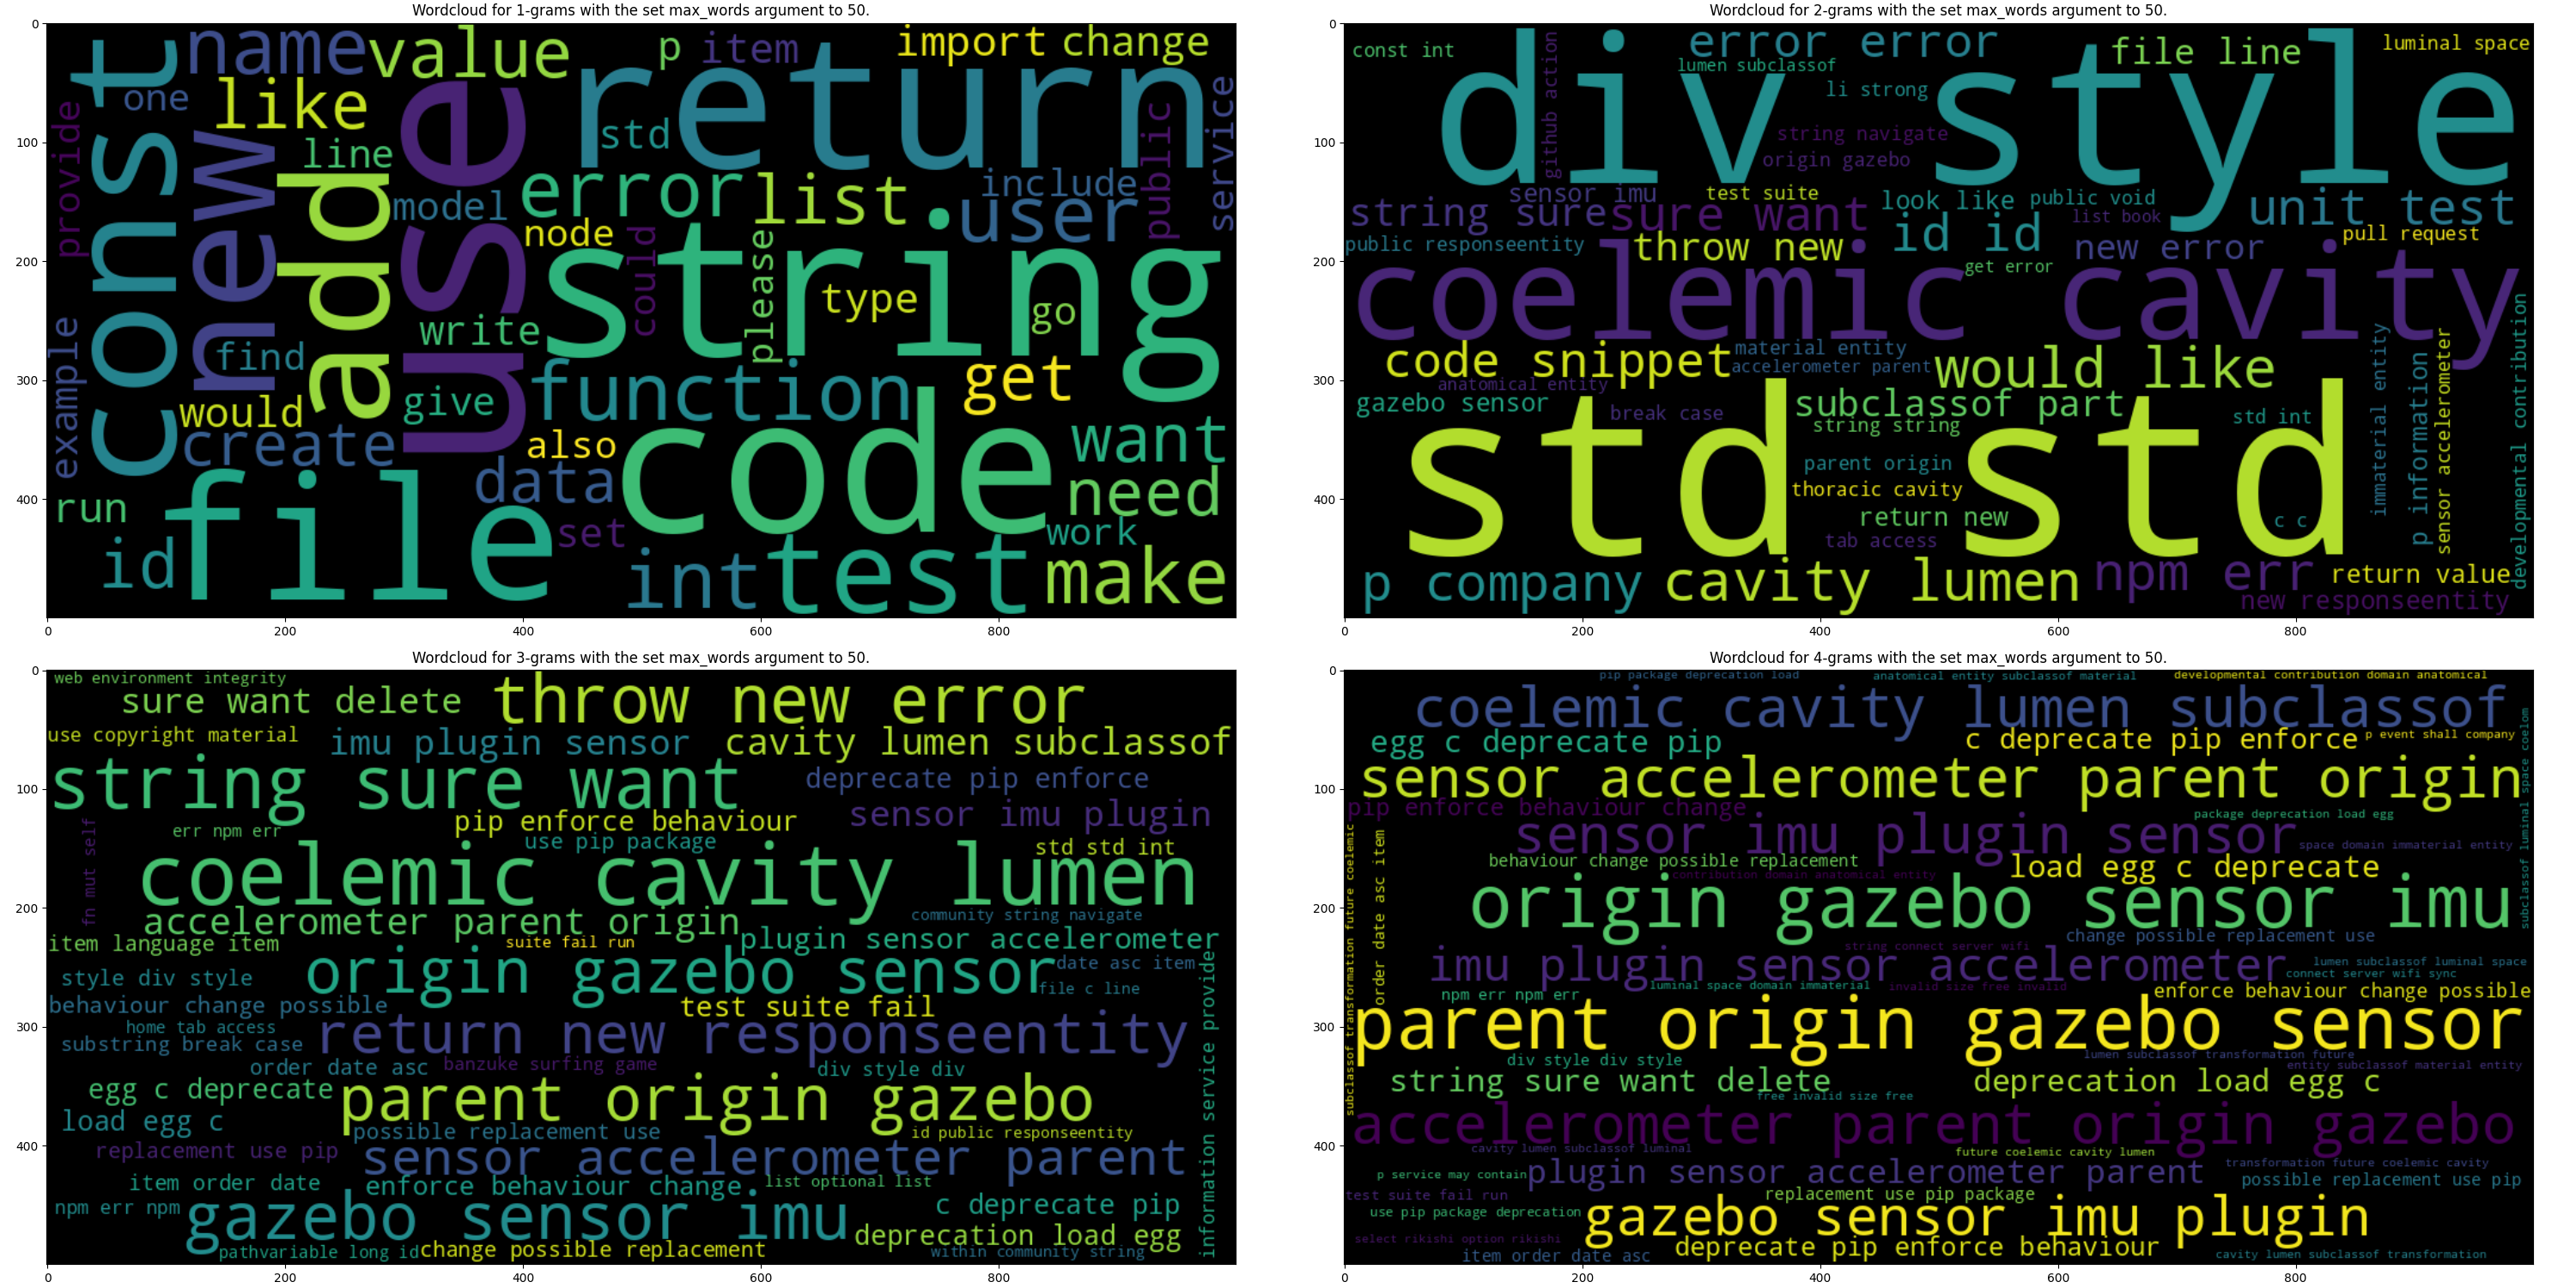
\includegraphics[width=\textwidth]{imgs/pull_requests-ngrams.png}
    \caption{N-grams from conversations sourced from GitHub pull requests.}
    \label{fig:pr-ngrams}
\end{figure}

\begin{figure}[H]
    \centering
    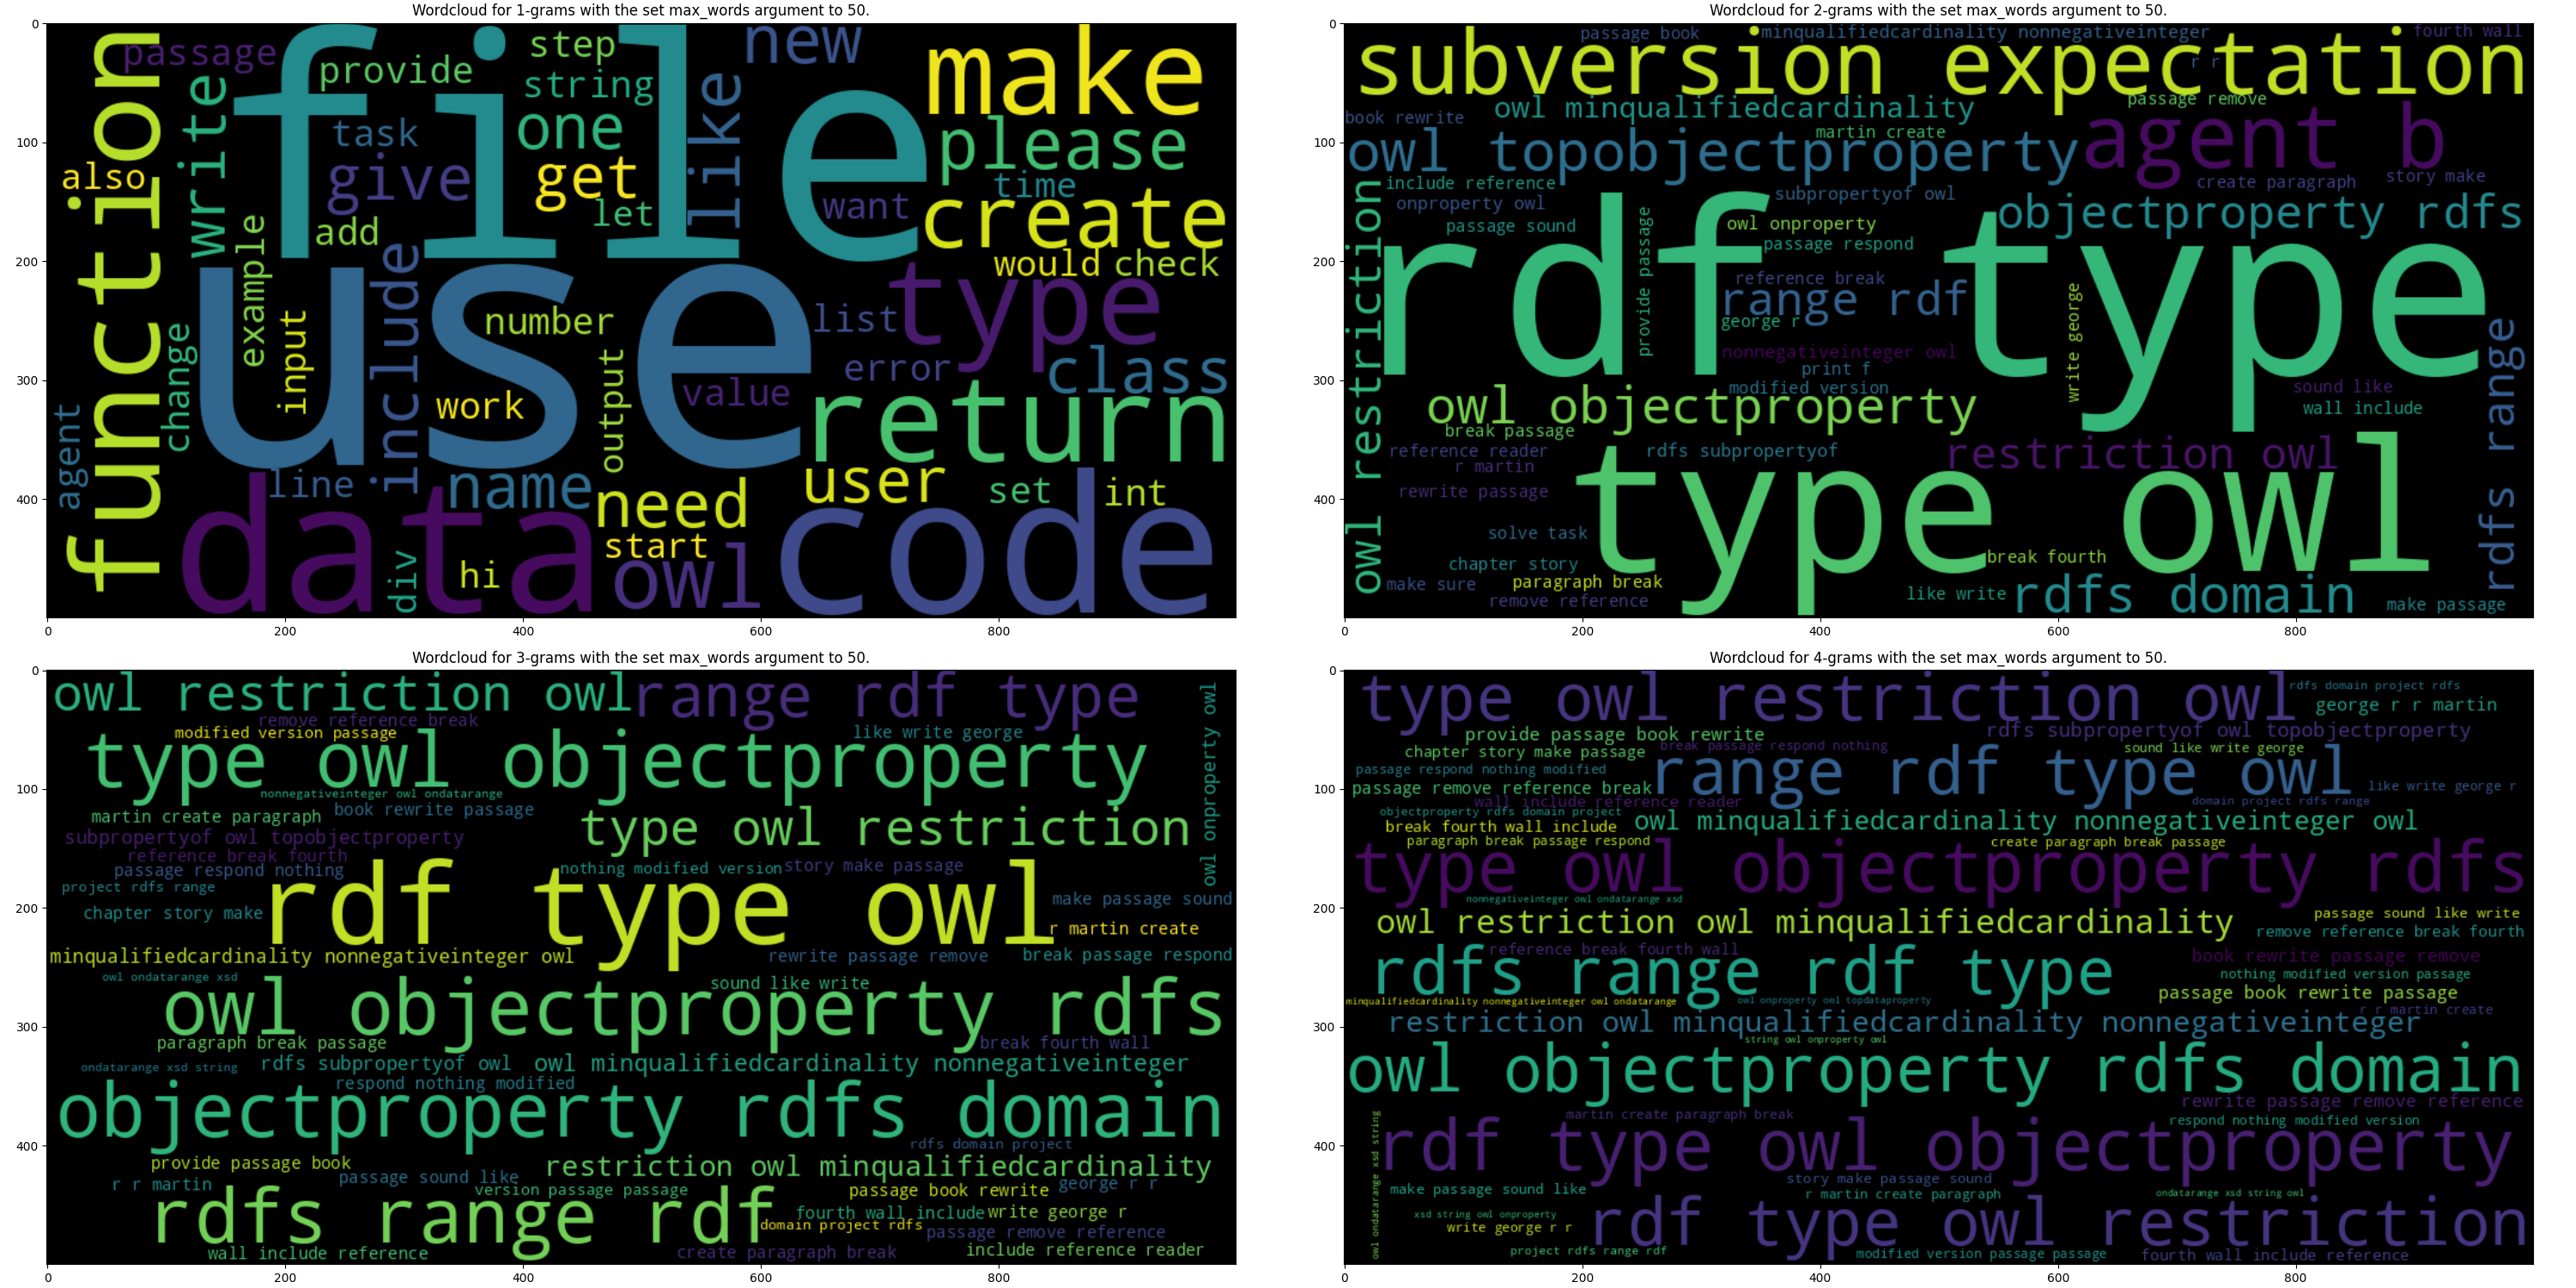
\includegraphics[width=\textwidth]{imgs/code_files-ngrams.png}
    \caption{N-grams from conversations sourced from GitHub code files.}
    \label{fig:code-ngrams}
\end{figure}

\begin{figure}[H]
    \centering
    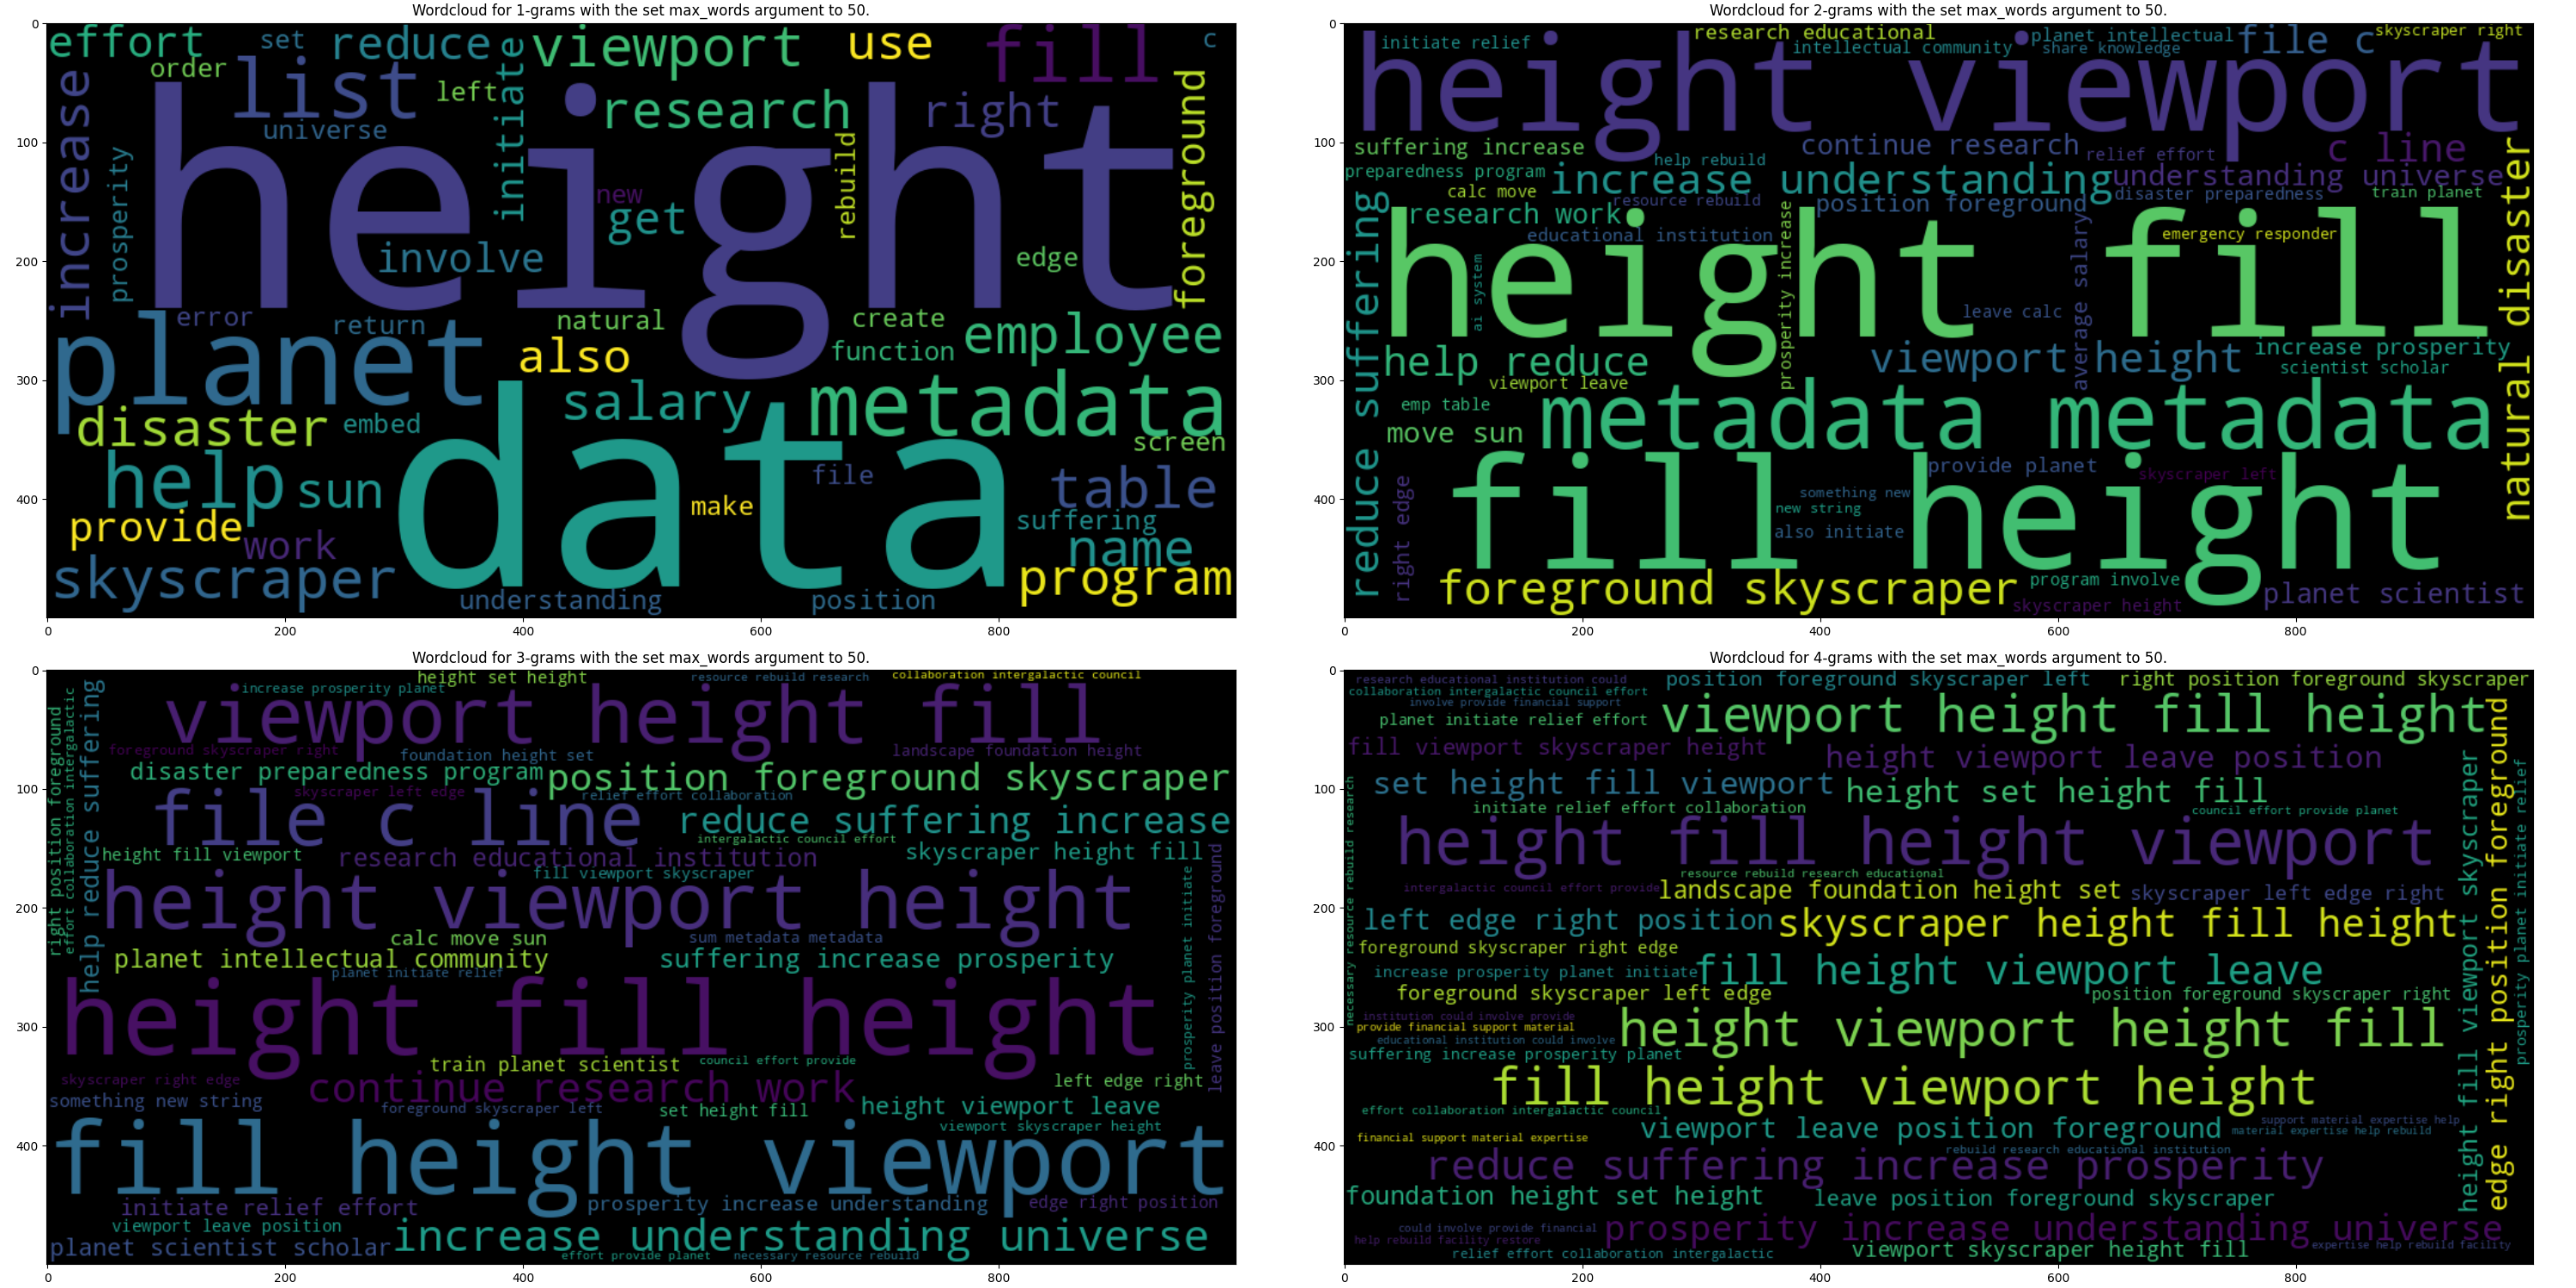
\includegraphics[width=\textwidth]{imgs/repository-ngrams.png}
    \caption{N-grams from conversations sourced from GitHub repositories.}
    \label{fig:repositories-ngrams}
\end{figure}

\begin{figure}[H]
    \centering
    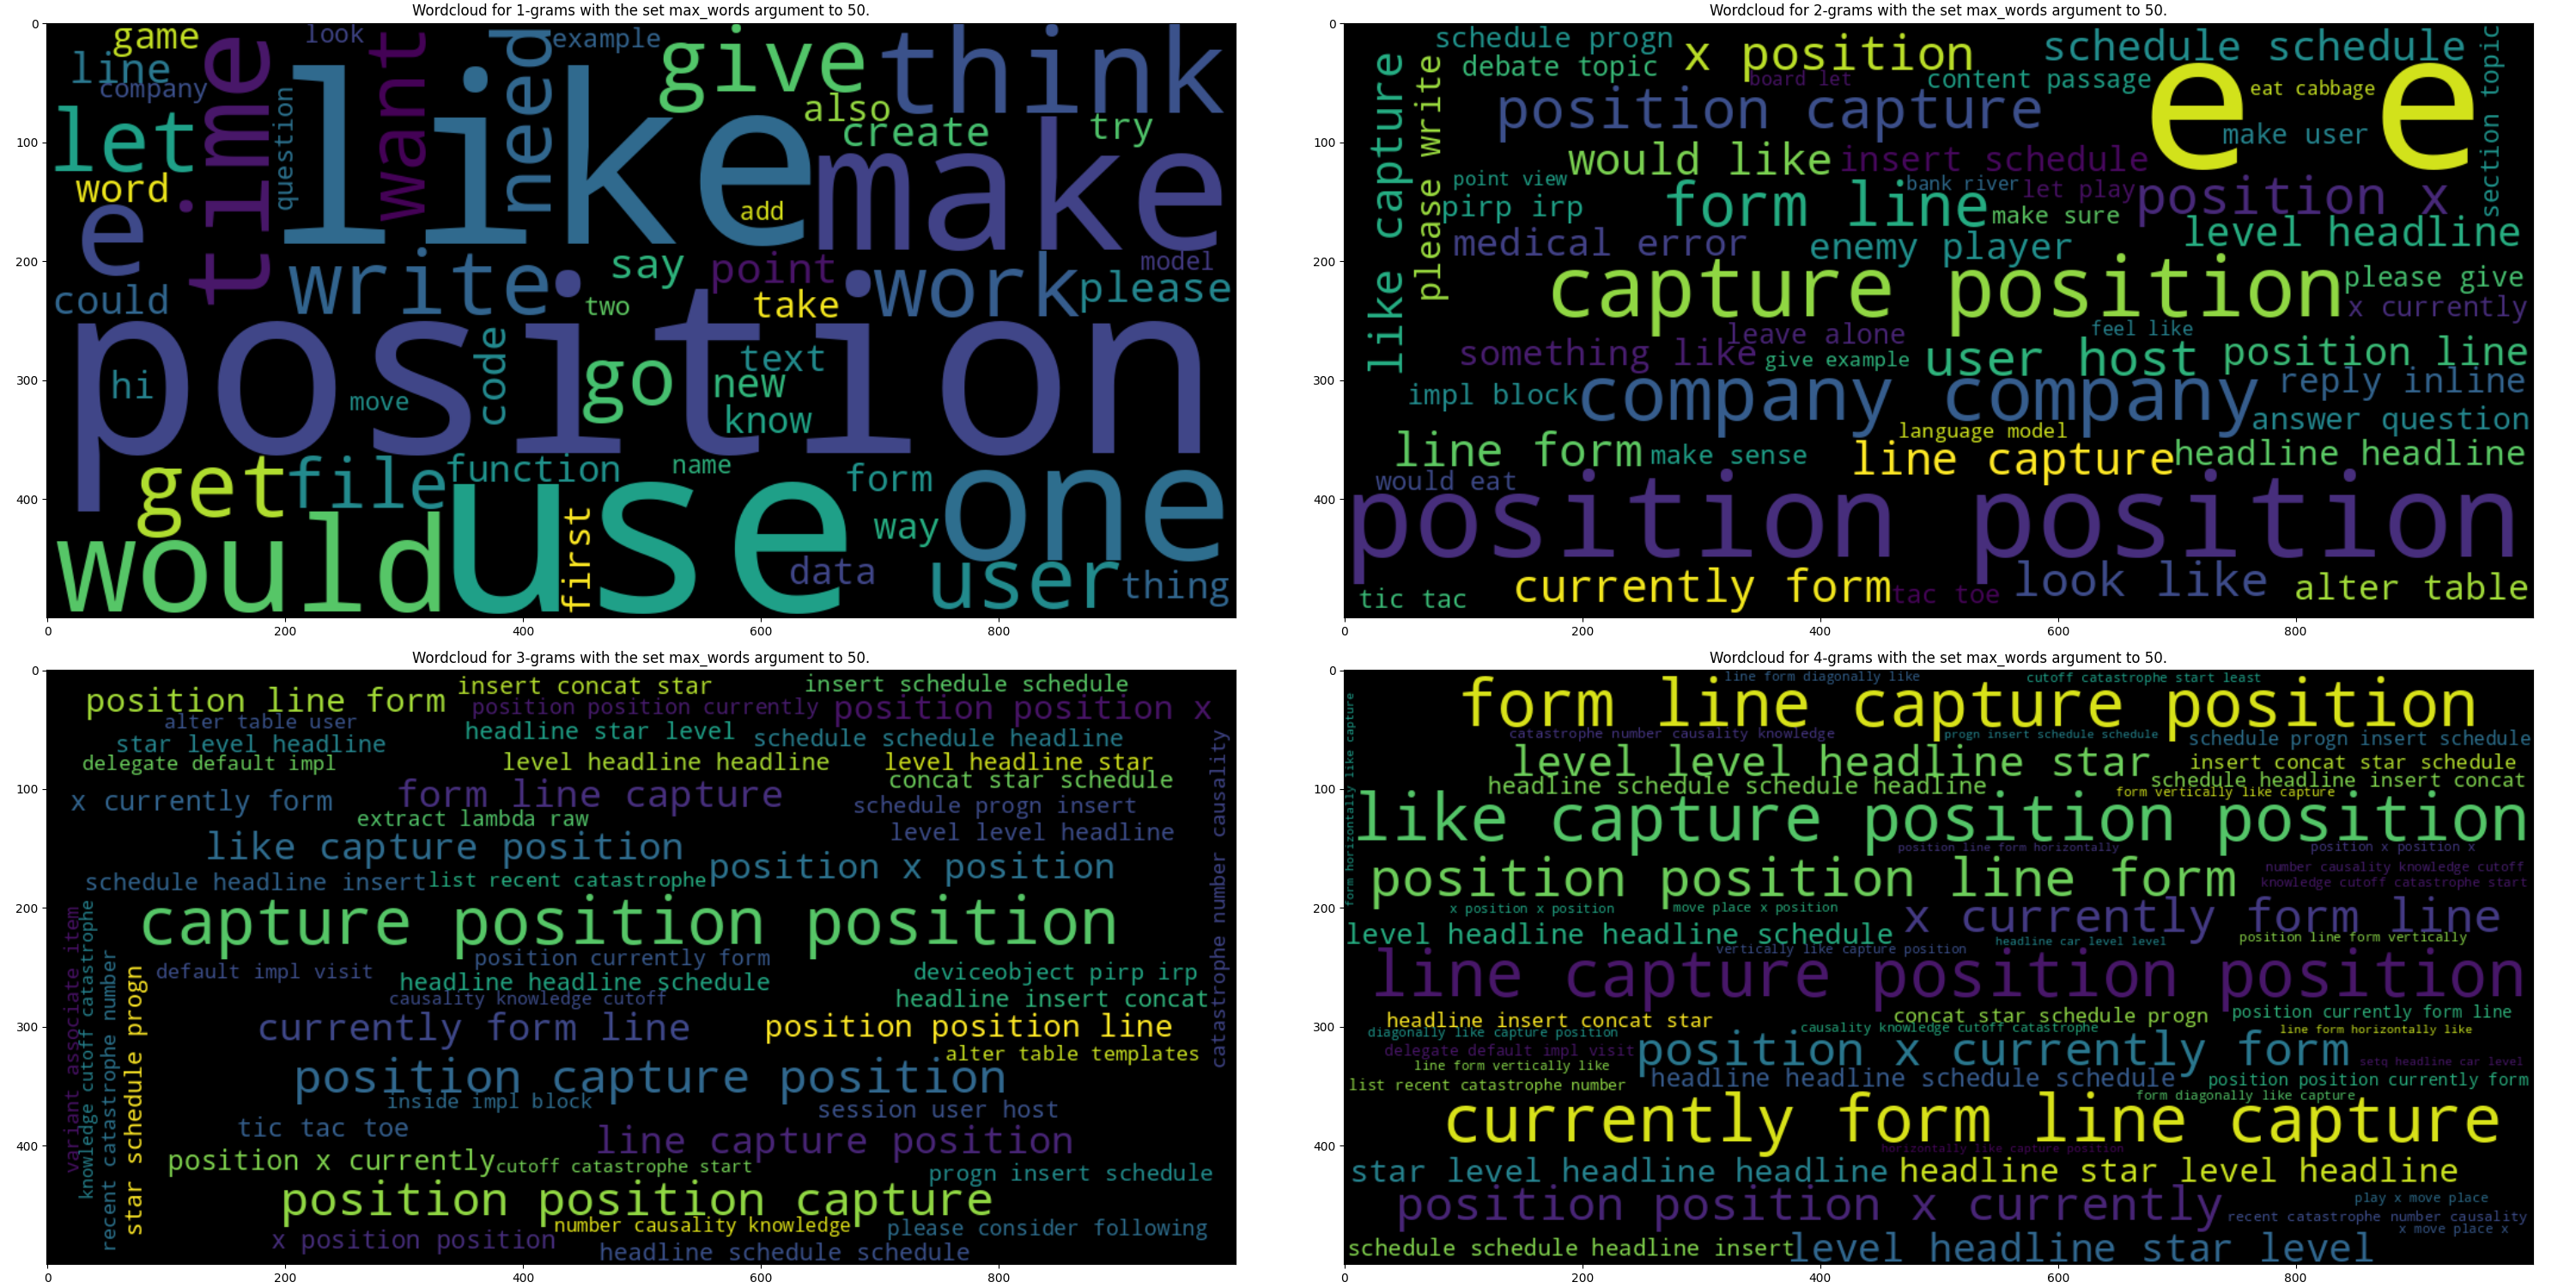
\includegraphics[width=\textwidth]{imgs/hacker_news-ngrams.png}
    \caption{N-grams from conversations sourced from Hacker News.}
    \label{fig:hn-ngrams}
\end{figure}

\pagebreak
\section{Topic models}\label{appendix:topic-models}

\begin{longtable}{|m{3cm}|m{9cm}|}
    \hline
    \textbf{Topic name} & \textbf{Top words}  \\
    \hline
    \hline
        Task-based file management & file, task, need, set, solve, solve task, use, working set, working, create \\
    \hline
        Function testing & test, use, file, name, code, find, std, return, gettile, tile \\
    \hline
        UI layout planning & plan, file, height, use, create, div, script, goal, go, import \\
    \hline
        AI-assisted development & file, task, use, junior, prompt, ai, project, create, work, script \\
    \hline
\caption{Topic models with top words for conversations sourced from GitHub commits.}
\label{table:commits-topics}
\end{longtable}

\begin{longtable}{|m{4cm}|m{8cm}|}
    \hline
    \textbf{Topic name} & \textbf{Top words}  \\
    \hline
    \hline
        Code \& model behavior & use, file, th, return, line, code, model, input, error, string \\
    \hline
        Data \& value processing & use, file, return, show, name, process, value, number, function, string \\
    \hline
\caption{Topic models with top words for conversations sourced from GitHub issues.}
\label{table:issues-topics}
\end{longtable}

\begin{longtable}{|m{4cm}|m{8cm}|}
    \hline
    \textbf{Topic name} & \textbf{Top words}  \\
    \hline
    \hline
        Product design feasibility & desirability, feasibility, customer, episode, technology, operational, technology feasibility, customer desirability, employee desirability, employee \\
    \hline
        Silicon Valley series & richard, pied, pied piper, piper, hi, use, hooli, file, erlich \\
    \hline
        Data handling & object, use, string, try short string, environment, email, want, agent, json, data \\
    \hline
        Node installation issues & new, node, value, error, please, install, npm, run, path \\
    \hline
        Change history & change, file, type, use, team, write, history, device, change history \\
    \hline
        Silicon Valley cast & hi, richard, belson, erlich, piper, pied piper, app, dinesh, gilfoyle \\
    \hline
        Messages \& Actions & richard, say, return, hi, message, use, action, code, student, pied \\
    \hline
        Silicon Valley series: Pied Piper & richard, pied, pied piper, piper, use, hi, hooli, clause, service \\
    \hline
        Model calibration & agent, tool, model, policy, use, experiment, calibration \\
    \hline
\caption{Topic models with top words for conversations sourced from GitHub discussions.}\label{table:discussions-topics}
\end{longtable}

\begin{longtable}{|m{5cm}|m{7cm}|}
    \hline
    \textbf{Topic name} & \textbf{Top words}  \\
    \hline
    \hline
        C++ function signatures & return, std, string, use, value, int, vector, const, line, file \\
    \hline
        Node package metadata & use, author, node, npm, list, resource, id, code, file, return \\
    \hline
        Ontology \& classification & subclassof, id, string, cavity, entity, return, book, genre, part, use \\
    \hline
        Mathematical constants \& Types & const, sum, code, int, use, false, list, float, function, add \\
    \hline
        Web attestation APIs & string, use, user, code, return, attestation, like, web, request, attester \\
    \hline
        Item handling logic & item, use, string, want, code, need, file, function, please, return \\
    \hline
        Python packaging errors & program, pip, use, write, package, error, user, go, memory, model \\
    \hline
        Enterprise service logic & service, company, code, use, make, information, std, go, provide, get \\
    \hline
        File-based testing & use, test, file, add, run, function, image, style, echo, code \\
    \hline
        Module initialization errors & new, const, code, error, import, string, id, return, public, list \\
    \hline
\caption{Topic models with top words for conversations sourced from GitHub pull requests.}
\label{table:pr-topics}
\end{longtable}

\pagebreak

\begin{longtable}{|m{4cm}|m{8cm}|}
    \hline
    \textbf{Topic name} & \textbf{Top words}  \\
    \hline
    \hline
        Step-by-step coding guidance & say, code, step, please, std, style, solution, end, use, detail \\
    \hline
        Evidence-supported argument & agent, argument, please, topic, subject, student, evidence, make, workshop, debate \\
    \hline
        Book passage creation & like, passage, use, make, hi, would, one, know, provide, time \\
    \hline
        OWL/RDF ontologies & owl, type, rdfs, rdf, rdf type, class, rdf type owl, type owl, relationship, ontology \\
    \hline
        Functional file operations & file, use, return, function, code, data, new, create, int, error \\
    \hline
\caption{Topic models with top words for conversations sourced from GitHub code files}
\label{table:code-files-topics}
\end{longtable}

\begin{longtable}{|m{4cm}|m{8cm}|}
    \hline
    \textbf{Topic name} & \textbf{Top words}  \\
    \hline
    \hline
        UI layout metadata & height, metadata, list, skyscraper, viewport, fill, height fill, data, employee, salary \\
    \hline
        Research effort & planet, help, disaster, increase, research, program, also, reduce, effort, data \\
    \hline
\caption{Topic models with top words for conversations sourced from GitHub repositories.}
\label{table:repository-topics}
\end{longtable}


\begin{longtable}{|m{4cm}|m{8cm}|}
    \hline
    \textbf{Topic name} & \textbf{Top words}  \\
    \hline
    \hline
        Conversational requests & could, would, hi, make, go, time, question, one, use, like \\
    \hline
        User-host session actions & make, user, host, write, user host, word, goal, please, get, like \\
    \hline
        Narrative creation & one, story, use, like, hi, would, give, create, question, think \\
    \hline
        Game interraction errors & one, give, like, game, use, add, code, medical, error, would \\
    \hline
        File tracking utilities & use, track, let, file, return, like, one, time, point, value \\
    \hline
        Company schedule & company, company company, company company company, company company company company, headline, schedule, insert, level, like, tell \\
    \hline
        Positional pattern capture & position, position position, position position position, like, capture, capture position, capture position position, capture position position position, line, form \\
    \hline
        Code support & use, make, get, time, work, one, code, like, need, give \\
    \hline
\caption{Topic models with top words for conversations sourced from HackerNews.}
\label{table:hn-topics}
\end{longtable}

\pagebreak
\section{Topic models' WordClouds}\label{appendix:topic-models-wordclouds}

\begin{figure}[H]
    \centering
    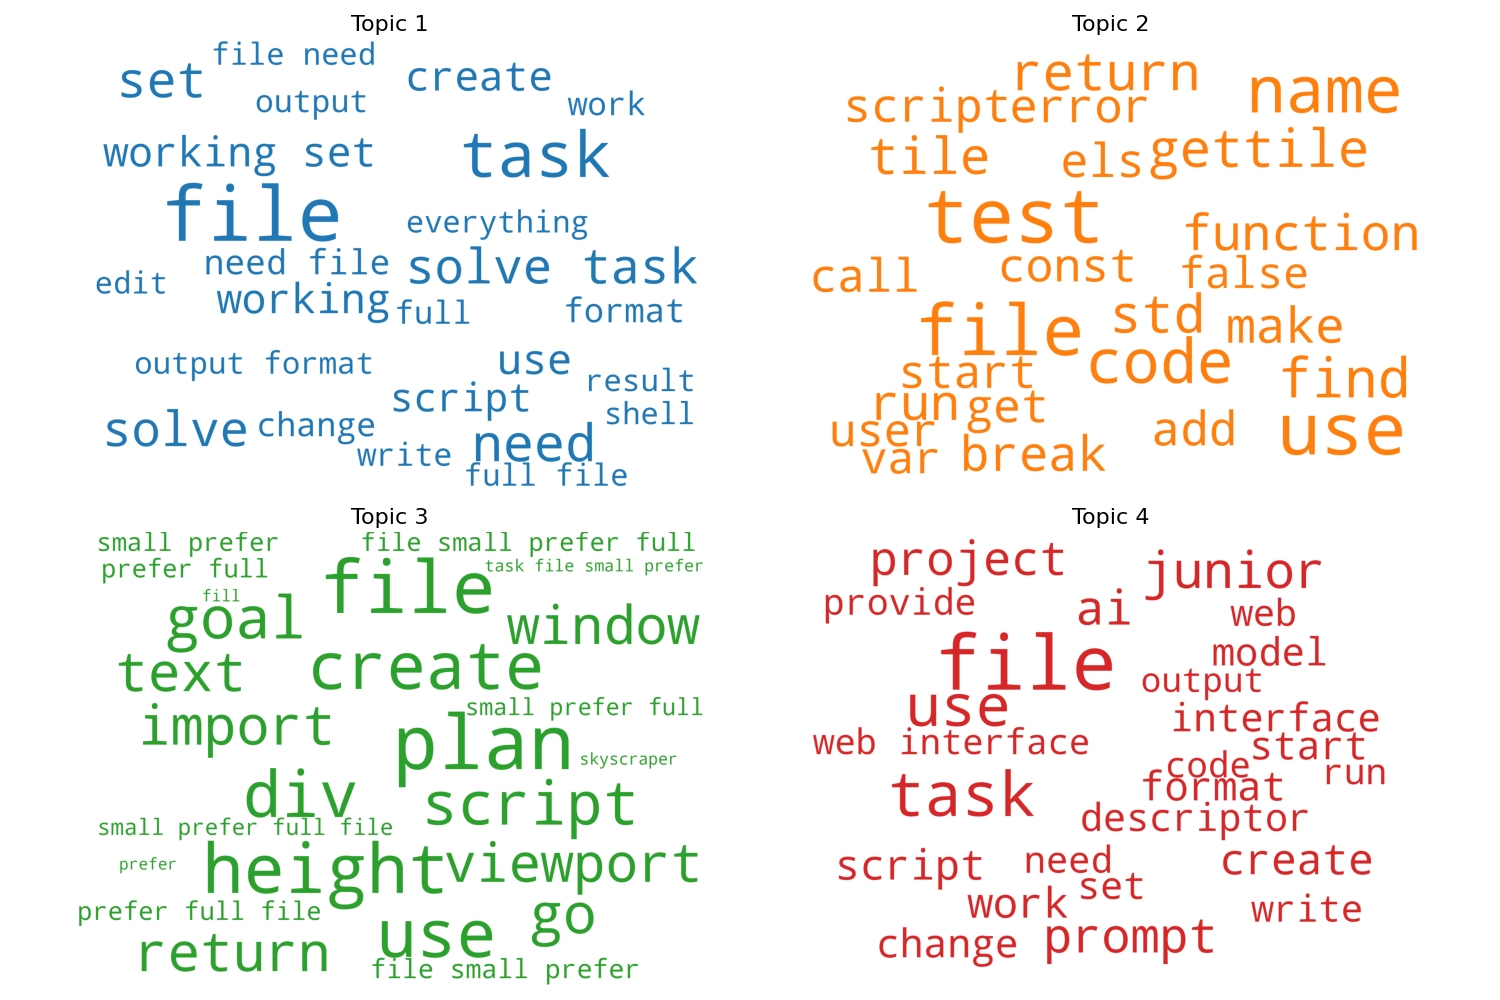
\includegraphics[width=\textwidth]{imgs/commits-topic-modelling.png}
    \caption{Topic models for conversations sourced from GitHub commits.}
    \label{fig:commits-topic-modelling}
\end{figure}

\begin{figure}[H]
    \centering
    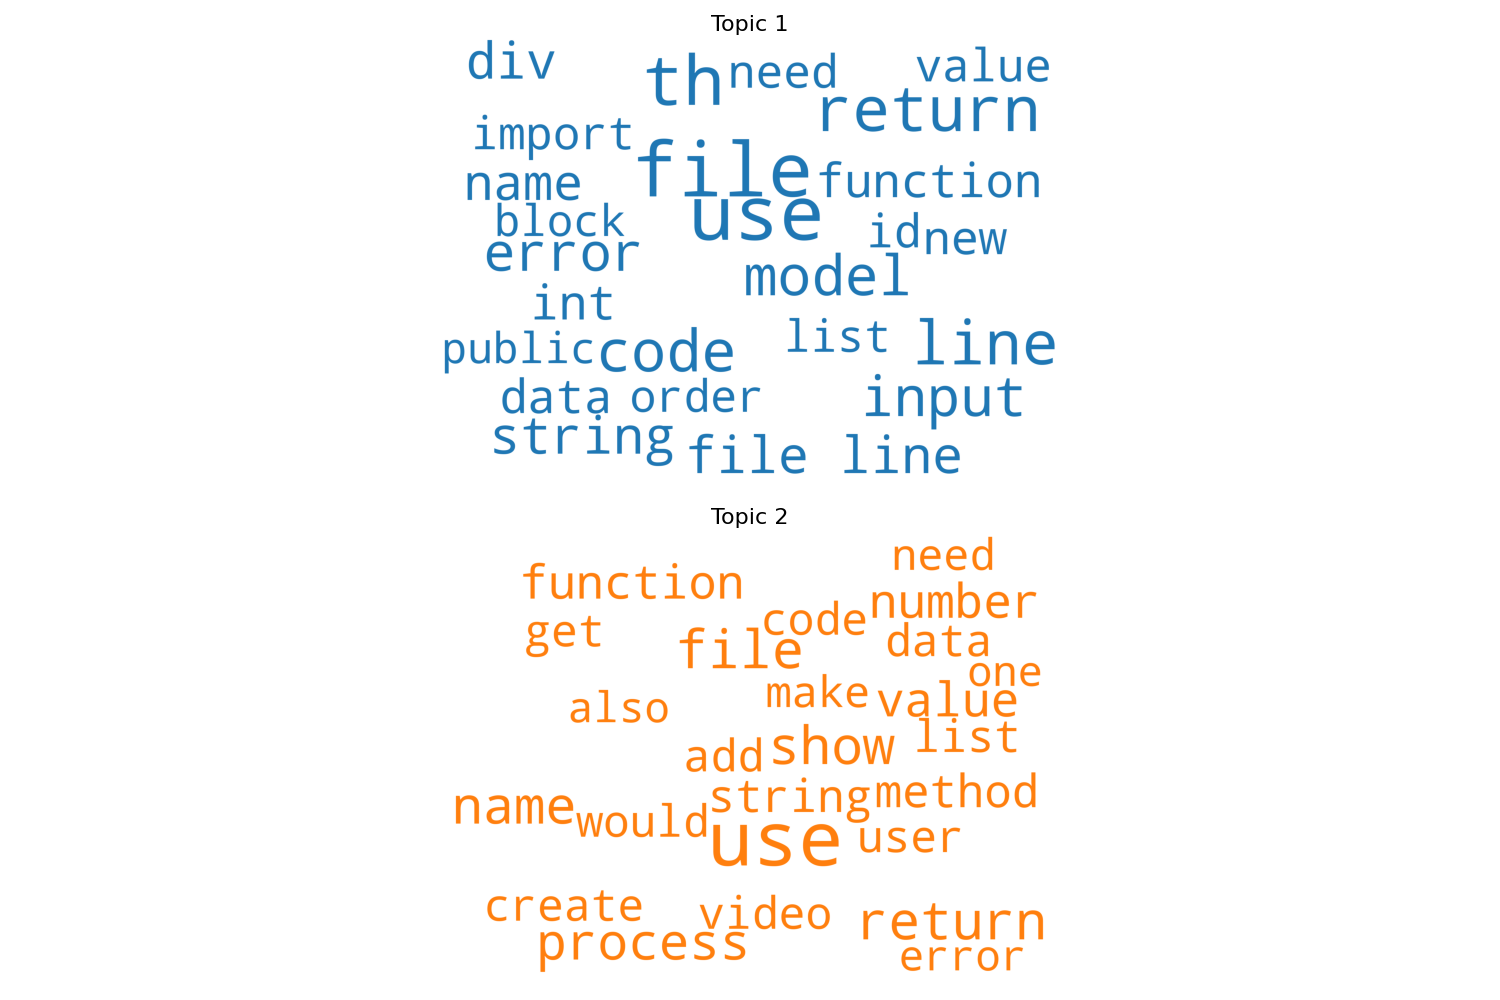
\includegraphics[width=\textwidth]{imgs/issues-topic-modelling.png}
    \caption{Topic models for conversations sourced from GitHub issues.}
    \label{fig:issues-topic-modelling}
\end{figure}

\begin{figure}[H]
    \centering
    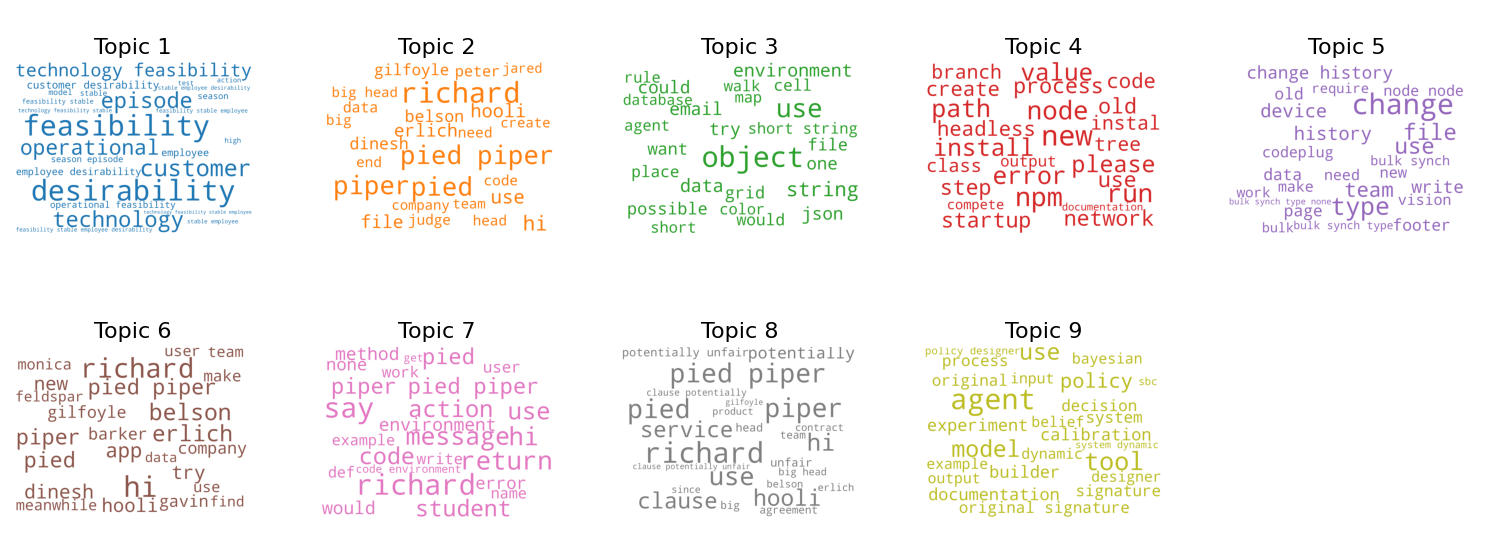
\includegraphics[width=\textwidth]{imgs/discussions-topic-modelling.png}
    \caption{Topic models for conversations sourced from GitHub discussions.}
    \label{fig:discussions-topic-modelling}
\end{figure}

\begin{figure}[H]
    \centering
    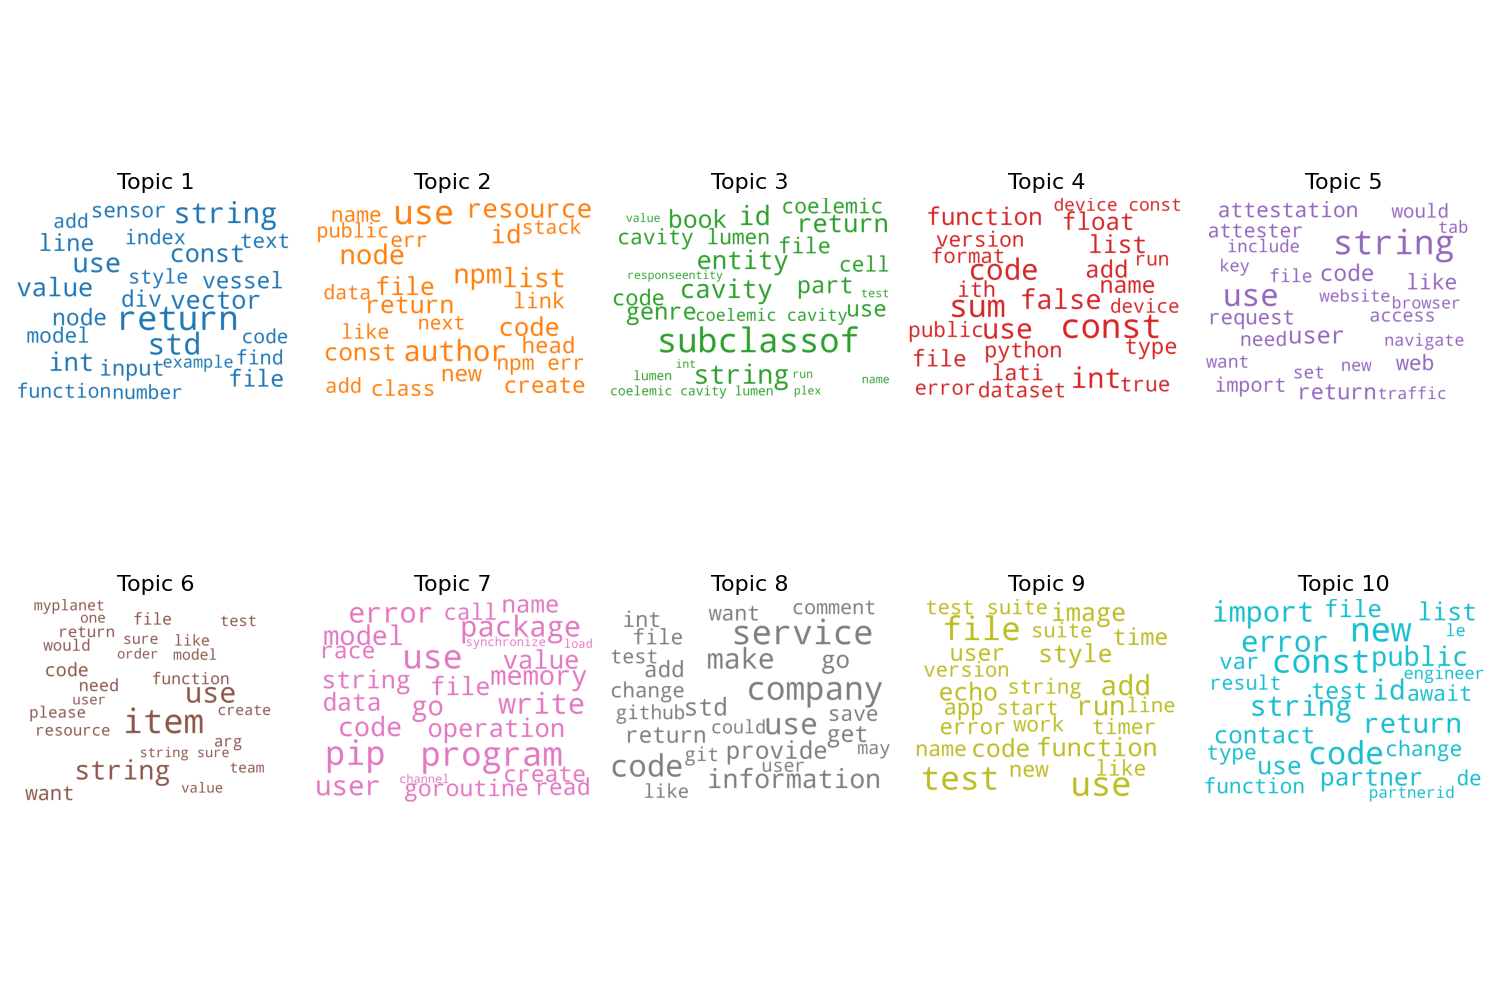
\includegraphics[width=\textwidth]{imgs/pull_requests-topic-modelling.png}
    \caption{Topic models for conversations sourced from GitHub pull requests.}
    \label{fig:pr-topic-modelling}
\end{figure}

\begin{figure}[H]
    \centering
    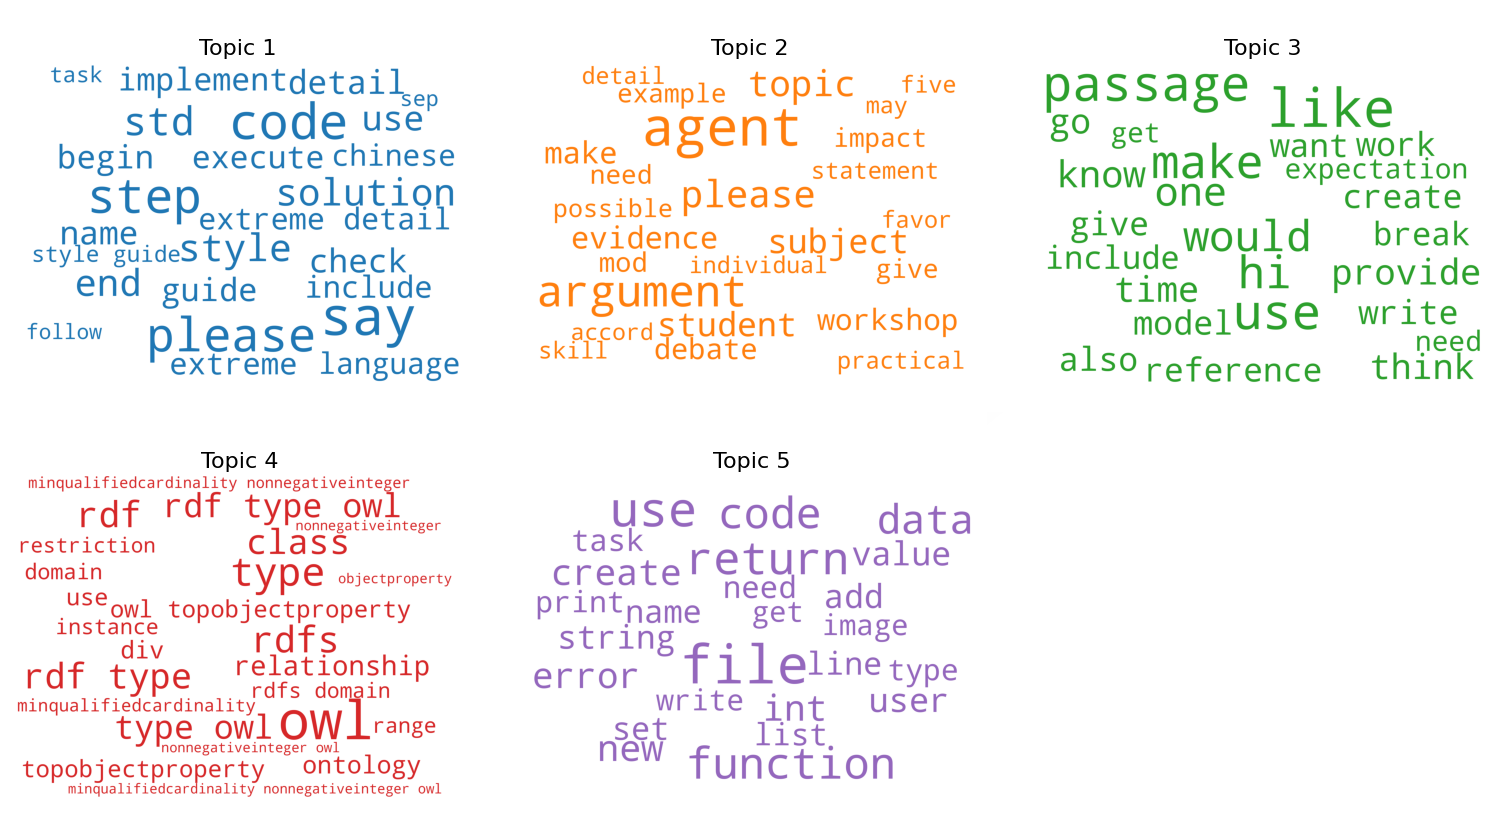
\includegraphics[width=\textwidth]{imgs/code_files-topic-modelling.png}
    \caption{Topic models for conversations sourced from GitHub code files.}
    \label{fig:code-topic-modelling}
\end{figure}

\begin{figure}[H]
    \centering
    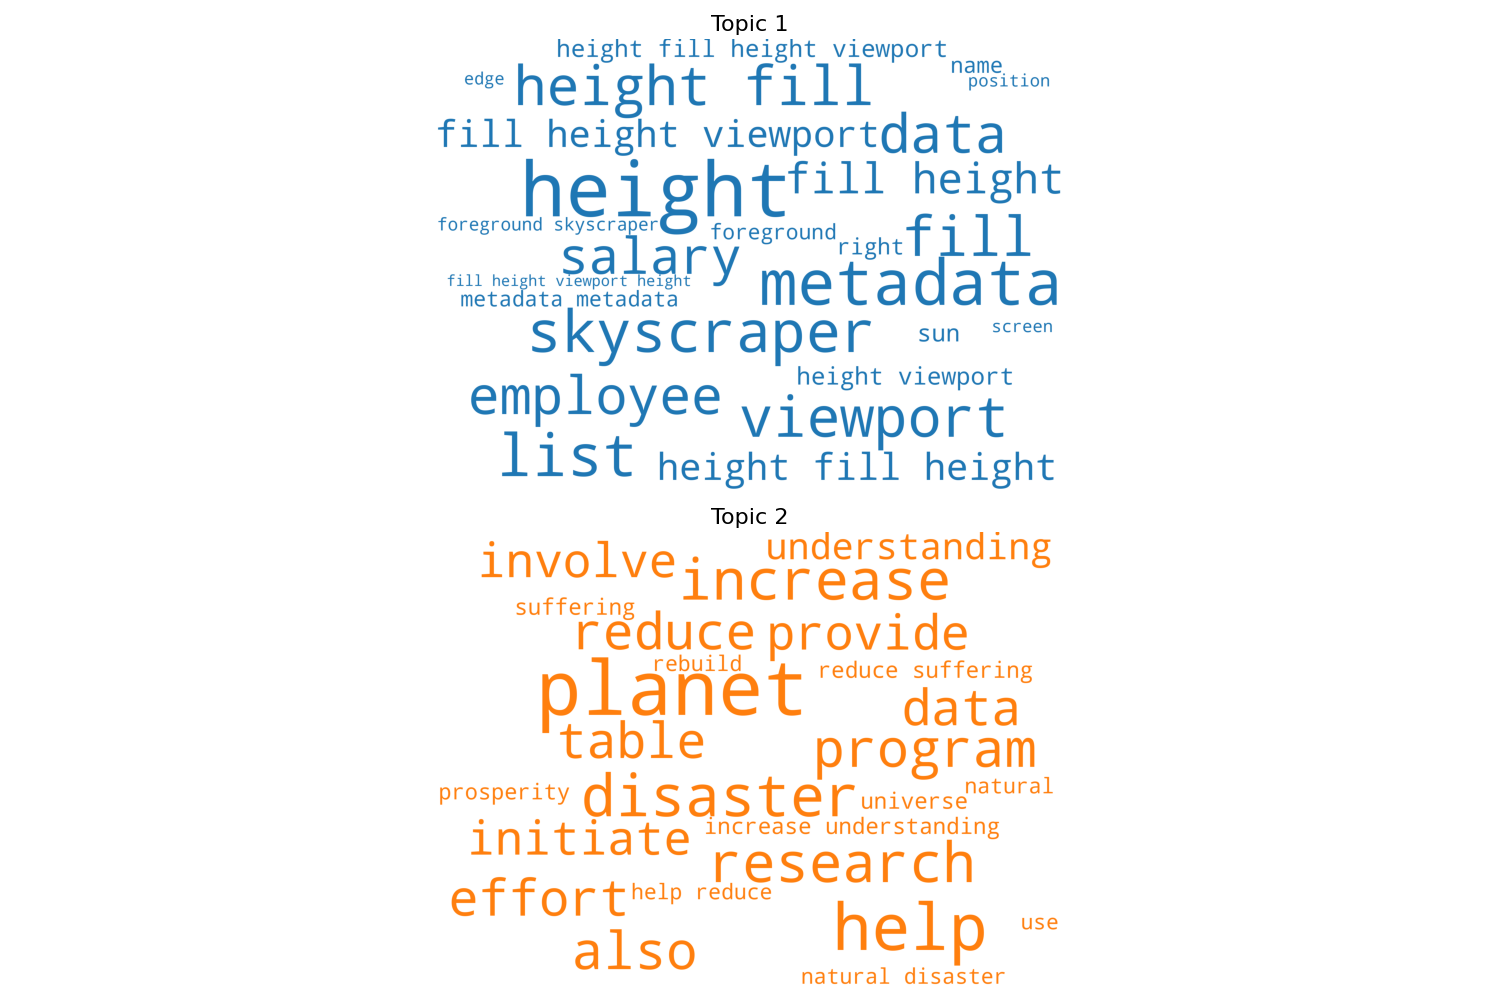
\includegraphics[width=\textwidth]{imgs/repository-topic-modelling.png}
    \caption{Topic models for conversations sourced from GitHub repositories.}
    \label{fig:repositories-topic-modelling}
\end{figure}

\begin{figure}[H]
    \centering
    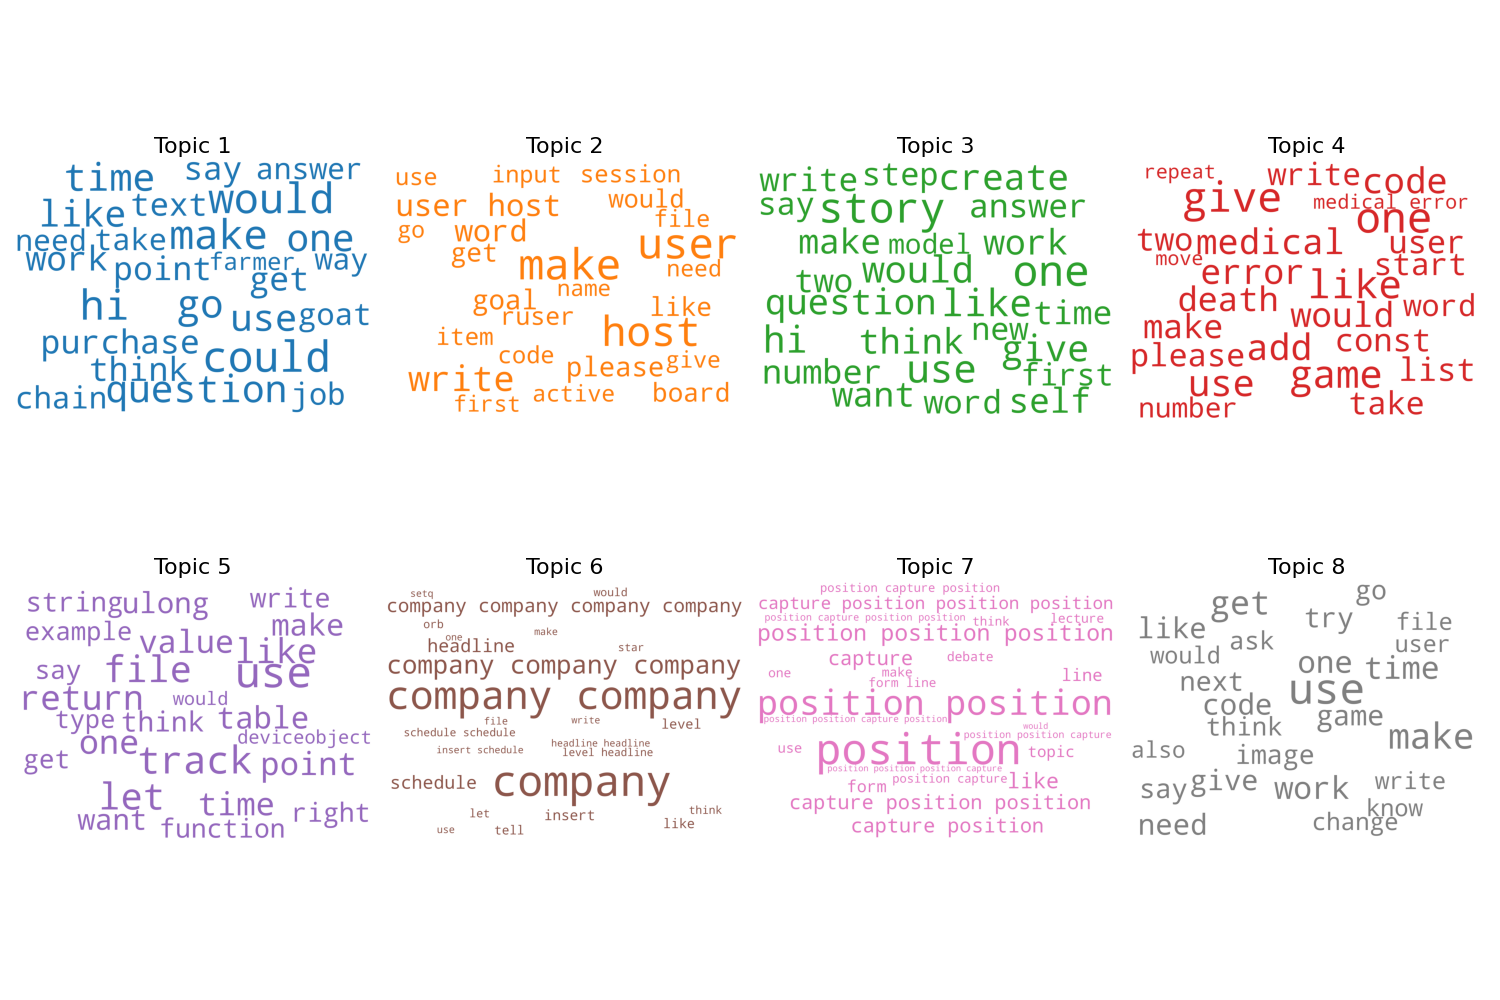
\includegraphics[width=\textwidth]{imgs/hacker_news-topic-modelling.png}
    \caption{Topic models for conversations sourced from Hacker News.}
    \label{fig:hn-topic-modelling}
\end{figure}